\chapter{Monte Carlo techniques}\label{chap:2}


\section{Mothecarlo Technique DA COMPLETARE MATIAS}

\subsection{Random Number}
With hindsight, it seems clear that the whole field of random number generation
was mesmerized, for far too long, by the simple recurrence equation:
\begin{equation}
I_{i+1} = aI_{i} + b \pmod{m}
\label{eq:1}
\end{equation}


Here m is called the modulus, a is a positive integer called the multiplier, and c
(which may be zero) is nonnegative integer called the increment. For c different from 0, the equation is called a linear congruential generator (LCG). When c is equal to 0, it is sometimes
called a multiplicative LCG or MLCG.
The recurrence \ref{eq:1} must eventually repeat itself, with a period that is obviously no greater than m. If m; a; and c are properly chosen, then the period will be
of maximal length, i.e., of length m. In that case, all possible integers between 0 and
$m-1$ occur at some point, so any initial “seed” choice of I 0 is as good as any other:
The sequence just takes off from that point, and successive values I j are the returned
“random” values.
But there is a problem with the number obtained trough this procedure;if k random numbers at a time are used to plot points in k-dimensional space (with each coordinate between 0 and 1), then the points will not
tend to “fill up” the k-dimensional space, but rather will lie on $k-1$ dimensional
“planes”. There will be at most about $m^{1/k}$ such planes.If the constants m and a
are not very carefully chosen, there will be many fewer than that (for this reason this way is not used with Monte Carlo technique). The number m
was usually close to the machine’s largest representable integer, often $2^{32}$
(see pg345)
\begin{figure}[h!t]
\centering
\begin{subfigure}[ht]{0.45\textwidth}
	\centering
	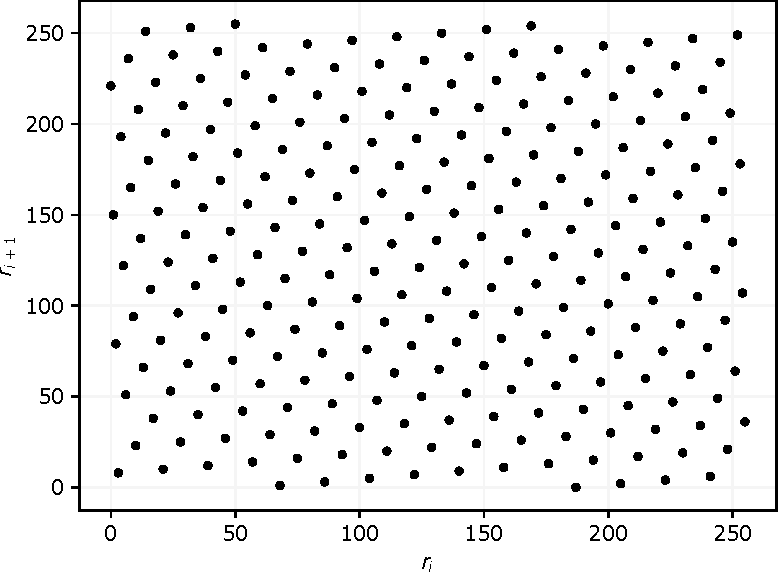
\includegraphics[width=\textwidth]{LCG}
	\caption{}\label{SpectralMethod2d}
\end{subfigure}
\hfill
\begin{subfigure}[ht]{0.51\textwidth}
	\centering
	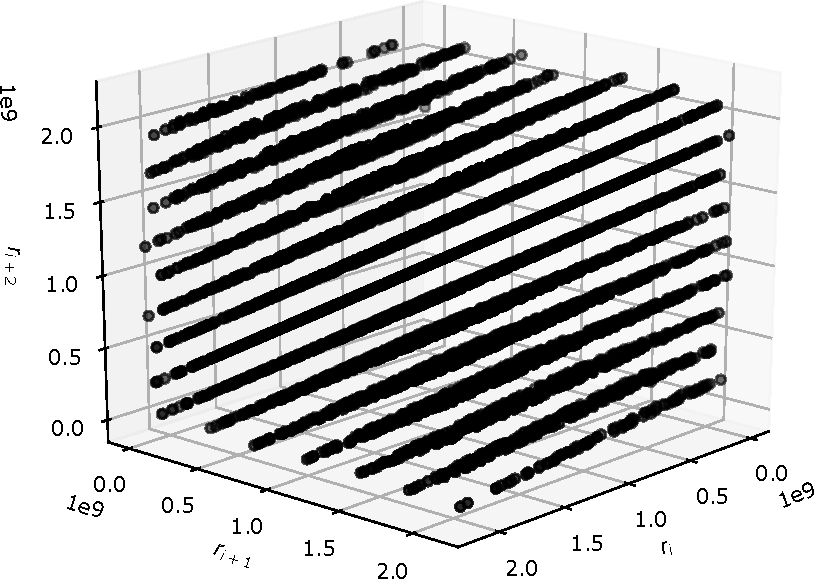
\includegraphics[width=\textwidth]{RANDU}
        \caption{}\label{SpectralMethod3d}
\end{subfigure}
\caption{\attachfile[icon=CustomPushPin,modified=20210303134907+01'00',size=377574]{Attachments/Spectral Test.ipynb} Examples of 2D (a) and 3D (b) spectral methods: (a) is set with $m=256$, $a=137$, $b=187$ (these parameters give full period), while (b) has $m=2^{31}$, $a=65539$, $b=0$ (this congruential generator is the (in)famous \texttt{RANDU}).}\label{SpectralMethod}
\end{figure}
\subsubsection{Ran0: the minimal standard}
NB di questa parte dobbiamo ancora prendere i riferimenti corretti

\subsection{Deviates from other distributions (from pg 361 num rec)}
Before, we learned how to generate random deviates with a uniform probability
between 0 and 1, denoted $U(0,1)$.
The probability of generating a number between
$x$ and $x+dx$ is
\[p(x)dx = \begin{cases}dx & 0 \le x < 1 \\ 0 & otherwise \end{cases}\]
Now we want generate random deviates drawn from other
probability distributions

\subsection{Exponential Deviates}
Suppose that we generate a uniform deviate $x$ and then take some prescribed
function of it, $y(x)$. The probability distribution of $y$, denoted $p(y)dy$, is determined
by the fundamental transformation law of probabilities, which is simply:
\[\left | p(y)dy \right |= \left | p(x)dx \right |\]
or 
\[\left | p(y)\right |= \left | p(x)\right | \left | \frac{dx}{dy} \right |\]
As example, take $y(x) = -\ln(x)$
We obtain:
\[\left | p(y)dy \right | = \left | \frac{dx}{dy} \right |dy = e^{-y}dy\]
NB $f^{-1}$ in this case is $x=e^{-y}$

I want number distributed as $e^{-y}$, so i generate random number (I know how do it), i take the $-\ln(x)$ of this number and what i obtain are numbers distributed exponentially. 

This distribution occurs frequently in real life, usually as the distribution of waiting times between independent Poisson-random events, for example the radioactive decay of nuclei.

\subsubsection{Transformation Method}
Best formalism can be found at:

\emph{\url{https://en.wikipedia.org/wiki/Inverse_transform_sampling}}


Let’s see what is involved in using the above transformation method to generate some arbitrary desired distribution of y’s, say one with $p(y)=f(y)$ for some positive function $f$ whose integral is 1. According to:
\[\left | p(y)\right |= \left | p(x)\right | \left | \frac{dx}{dy} \right |\]
we have to solve the equation:
\[ \frac{dx}{dy} = f(y) \]
but the solution of this equation is just $x=F(y)$ where $F(y)$ is the integral of $f(y)$. The desired transformation that takes a uniform deviate into one distributed as $f(y)$ is therefore: 
\[ y(x)=F^{-1}(x) \]
Since $F(y)$ is the area under the probability curve to the left of y, is just the prescription:
Choose a uniform random x, then find the value y that has that fraction x of probability area to its left, and return the value y.

\begin{figure}[h!t]
\centering
%\subfloat[][\emph{}]
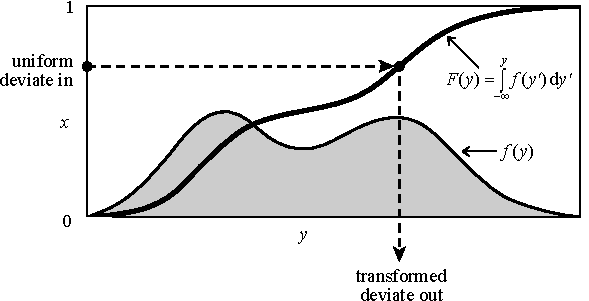
\includegraphics[scale=1]{Transformation Method}
\caption{Transformation method for generating a random deviate y from a known probability distribution $p(y)$. The indefinite integral of $p(y)$ must be known and invertible. A uniform deviate x is chosen between 0 and 1. Its corresponding y on the definite-integral curve is the desired deviate.}\label{fig:Transformation method}
\end{figure}

\subsection{Rejection Method}
The rejection method is a powerful, general technique for generating random deviates whose distribution function $p(x)dx$ (probability of a value occurring between x and $x+dx$) is known and computable.The rejection method does not require that the cumulative distribution function (indefinite integral of $p(x)$) be readily computable, much less the inverse of that function — which was required for the transformation method in the previous section.
The rejection method is based on a simple geometrical argument.

\begin{figure}[h!t]
\centering
\subfloat[][\emph{Rejection method for generating a random deviate x from a known probability distribution $p(x)$ that is everywhere less than some other function $p(x)$.The transformation method is first used to generate a random deviate x of the distribution f. A second uniform deviate is used to decide whether to accept or reject that x. If it is rejected, a new deviate of f is found, and so on.
The ratio of accepted to rejected points is the ratio of the area under p to the area between p and f}]
{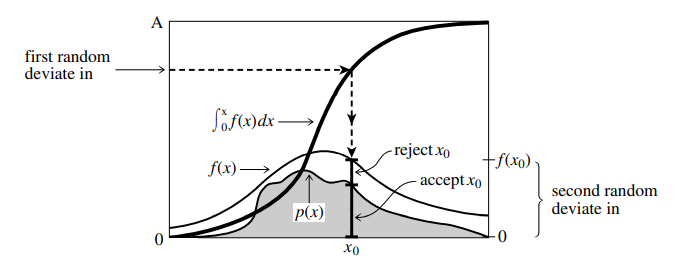
\includegraphics[width=.80\textwidth]{Rejection Method.PNG}}
\caption{}
\label{fig:Rejection method}
\end{figure}

Draw a graph of the probability distribution $p(x)$ that you wish to generate, so that the area under the curve in any range of x corresponds to the desired probability of generating an x in that range. If we had some way of choosing a random point in two dimensions, with uniform probability in the area under your curve, then the x value of that random point would have the desired distribution.

Now, on the same graph, draw any other curve f(x) that has finite (not infinite) area and lies everywhere above your original probability distribution. (This is always possible, because your original curve encloses only unit area, by definition of probability).We will call this $f(x)$ the \textbf{comparison function} . Imagine now that you have some way of choosing a random point in two dimensions that is uniform in the area under the comparison function. Whenever that point lies outside the area under the original probability distribution, we will reject it and choose another random point.
Whenever it lies inside the area under the original probability distribution, we will accept it.

\textbf{It should be obvious that the accepted points are uniform in the accepted area, so that their x values have the desired distribution.} It should also be obvious that the fraction of points rejected just depends on the ratio of the area of the comparison function to the area of the probability distribution function, not on the details of shape of either function.

It remains only to suggest how to choose a uniform random point in two dimensions under the comparison function $f(x)$. It is used a variant of the transformation method,\textbf{ be sure to have chosen a comparison function whose indefinite integral is known analytically, and is also analytically invertible to give x as a function of “area under the comparison function to the left of x.”} Now pick a uniform deviate between 0 and A, where A is the total area under $f(x)$, and use it to get a corresponding x.
Then pick a uniform deviate between 0 and $f(x)$ as the y value for the two-dimensional point. Finally, accept or reject according to whether it is respectively less than or greater than $p(x)$.

\subsection{Special Technique for Gaussian Distribution-Prof.}
Consider an ideal gas (compose by N), with whatever initial distribution of velocities. If the molecule can interact each other after a time interval $\Delta t$ they thermalized (they reach the thermodynamic equilibrium, so the distribution of the velocities is given by the Maxwell Boltzmann distribution: 
\[p(x) = \exp{\left(\frac{-E}{k_{\text{B}}T}\right)} = \exp{\left(\frac{-mv^2}{2k_{\text{B}}T}\right)}\]
This is the idea beyond this technique, we star from whatever distribution $f(x)$, and randomly pick up 2 particle ($j$ and $i$) from the gas (2 point in the interval and evaluate M.B.), then compute:
\[ v_{j}' = \frac{v_{j} + v_{i}}{\sqrt{2}} \]
\[ v_{i}' = \frac{v_{j} - v_{i}}{\sqrt{2}} \]

Now $v_{i}'$ and $v_{j}'$ are the \textbf{new velocities} of the particle $i$ and $j$, if you repeat the procedure a few time I'll end up with a Gaussian distribution (Maxwell Boltzmann in function of velocities)
if I have N particles the number of collision needed to thermalized is the order of $3N$ (so I have to repeat this procedure $3N$ times in a way of produce $N$ number distributed in a Gaussian Way).


\subsection{Metropolis Algorithm - Proof} 
The Metropolis algorithm is a general technique that allows to generate random number distributed according to a certain density probability $P(x)$ (it works even in more than 1 dimension). The Metropolis algorithm is based in few steps:

\newcounter{elenco}
\setcounter{elenco}{0}
\begin{list}{\stepcounter{elenco}\arabic{elenco}}{\setlength{\itemsep}{0.5cm}}
\item Generate a random number $x_n$.
\item Generate a new number $x_1$ through: $x_{n+1} = x_n + r \Delta$ where $r$ is a random number between $-1$ and $1$ and $\Delta$ is the typical scale on which the function $P(x)$ is changing (for example for a Gaussian is the variance).
N.B. $\Delta$ is the only information that we must have about the function $P(x)$. 
\item if $ f(x_{n+1}) > f(x_{n}) $ we always keep the point $x_{n+1}$\\
    if $ f(x_{n+1}) < f(x_{n}) $, compute the ratio $ R = \frac{f(x_{n+1})}{f(x_n)} $ of course $R \in \left[ 0,1 \right]$, now generate another pseudo random number $r' \in \left[ 0,1 \right]$, compare $R$ with $r'$  and if $ r'< R$ we keep $ x_{n+1} $ otherwise we reject $x_{n+1}$
\end{list}

We want show that if we repeat this procedure many times at the end the distribution of the points will reach an equilibrium an that this equilibrium correspond to the function P(x) .Now suppose that we have already generated $N$ points and we are moving them with the previous procedure and that $f(x)$ is a function proportional to $P(x)$. If we made a partition of the interval (in which in defined the function n) we can count the number of points in each interval (bin), so if $n_i$ are the points in the bin $i$, the variation of the number of point is $ \Delta n_i = n_j P_{ji} - n_i P_{ij}$ where $P_{ji}$ is the probability for a point in the bin $j$ to go in the bin $i$ and $P_{ij}$ is the probability for a point in the bin $i$ to go in the bin $j$. So we have: 
\[\Delta n_i = n_j P_{ij} \frac{P_{ji}}{P_{ij}} - \frac{n_i}{n_j}\]
\[ if \hspace{10pt} \frac{n_i}{n_j} > \frac{P_{ji}}{P_{ij}} \to \Delta n_i < 0 \]
Hence the system is evolving in a way that if we have too much points in $i$ the $\Delta n_i$ is negative (we are removing points from the bin $i$) and vice versa; so in this way a sort of equilibrium will be reach.
The probability $P_ij$ can be write as the product of 2 number, $ P_{ij} = g_{ij} A_{ij } $ where $g_{ij}$ is the probability that being in $i$ we generate a point in $i$ (we assume that $ g_{ij} = g_{ji} $) and $A_{ij}$ is the acceptance probability $A_{ij} = min \left\{1, \frac{f_j}{f_i} \right\}$ (so if $\frac{f_j}{f_i} > 1$ $A_{ij}$ is equal to one hence we always keep the new point compatible with what we said above), so from that we get:

\[ if \hspace{10pt} \frac{f_j}{f_i} < 1 \hspace{10pt} then \hspace{10pt}  A_{ij} = \frac{f_j}{f_i} \hspace{10pt} and \hspace{10pt} A_{ji} = 1 \hspace{10pt}\to \hspace{10pt} \frac{A_{ji}}{A_{ij}} = \frac{f_i}{f_j} \]
\[ if \hspace{10pt} \frac{f_j}{f_i} > 1 \hspace{10pt} then \hspace{10pt} A_{ij} = 1 \hspace{10pt} and \hspace{10pt} A_{ji} = \frac{f_i}{f_j} \hspace{10pt} \to \hspace{10pt} \frac{A_{ji}}{A_{ij}} = \frac{f_i}{f_j} \]

and finally,

\[ \frac{p_{ji}}{p_{ij}} = \frac{A_{ji}}{A_{ij}} = \frac{f_i}{f_j} \to \frac{n_i}{n_j} = \frac{f_i}{f_j} \]

therefore we are generating points according the function $f(x)$.

Code: Area of the circle, IdealGas-MarkovChain.  

\subsection{Simulated annealing}
\textit{The method of simulated annealing} is a technique that has attracted significant attention as suitable for optimization problems of large scale, especially ones where a desired global extremum is hidden among many poorer, local extrema. For practical purposes, simulated annealing has effectively “solved” the famous traveling salesman problem of finding the shortest cyclical itinerary for a traveling salesman who must visit each of N cities in turn and the problem of the arrangement of several hundred thousand circuit elements on a tiny silicon substrate is optimized so as to minimize interference among their connecting wires.
Notice that the two applications cited are both examples of combinatorial minimization. There is an objective function to be minimized, as usual, but the space over which that function is defined is not simply the N-dimensional space of $N$ continuously variable parameters. Rather, it is a discrete, but very large, configuration space, like the set of possible orders of cities, or the set of possible allocations of silicon "real estate” blocks to circuit elements.
At the heart of the method of simulated annealing is an analogy with thermodynamics, specifically with the way that liquids freeze and crystallize or metals cool and anneal. At high temperatures, the molecules of a liquid move freely with respect to one another. If the liquid is cooled slowly, thermal mobility is lost. The atoms are often able to line themselves up and form a pure crystal that is completely ordered over a distance up to billions of times the size of an individual atom in all directions. This crystal is the state of minimum energy for this system. The amazing fact is that, for slowly cooled systems, nature is able to find this minimum energy state. In fact, if a liquid metal is cooled quickly or “quenched,” it does not reach this state but rather ends up in a polycrystalline or amorphous state having somewhat higher energy.
 The so-called Boltzmann probability distribution,
 \[ P(E) \sim \exp(-E/KT) \]
expresses the idea that a system in thermal equilibrium at temperature T has its energy probabilistically distributed among all different energy states E. Even at low temperature, there is a chance, albeit a very small one, of a system being in a high energy state. Therefore, there is a corresponding chance for the system to get out of a local energy minimum in favor of finding a better, more global one. In other words, the system sometimes goes uphill as well as downhill; but the lower the temperature, the less likely is any significant uphill excursion.
N.B The crutial idea is that \textit{to minimize E means to maximize $P(E)$}

Code: Simulated-Annealing.

Pag. 825 Numerical Recipes 
Simulated Annealing pag 549 Numerical recipes: way to use a global minimum in triky situation, without getting stuck.

\subsubsection{Traveling Salesman with Metropolis}

%\newcounter{elenco}
%\setcounter{elenco}{0}
%\begin{list}{\stepcounter{elenco}\arabic{elenco}}{\setlength{\itemsep}{0.5cm}}
\begin{enumerate}
\item \textit{Configuration.} The cities are numbered $i = 1,\dots,N$ and each has coordinates $(x_i,y_i)$. A configuration is a permutation of the number $1,\dots,N$, interpreted as the order in which the cities are visited.
\item \textit{Rearrangements.} An efficient set of moves has been suggested by Lin, (Lin, S. 1965, “Computer Solutions of the Traveling Salesman Problem,” Bell System Technical Journal, vol. 44, pp. 2245–2269). The moves consist of two types: (i) A section of path is removed and then replaced with the same cities running in the opposite order; or (ii) a section of path is removed and then replaced in between two cities on another, randomly chosen, part of the path.
\item Objective function. In the simplest form of the problem, E is taken just as the total length of the journey,
\[ E = L \equiv \sum_{i=0}^{N-1} \sqrt{(x_i-x_{i+1})^2+(y_i-y_{i+1})^2}  \]
with the convention that point N is identified with point 0. To illustrate the flexibility of the method, however, we can add the following additional wrinkle: Suppose that the salesman has an irrational fear of flying over the Missisippi River. In that case, we would assign each city a parameter $\mu_i$ , equal to $+1$ if it is east of the Mississippi and $-1$ if it is west, and take the objective function to be
\[ E = L \equiv \sum_{i=0}^{N-1} \sqrt{(x_i-x_{i+1})^2+(y_i-y_{i+1})^2} + \lambda(\mu_i - \mu_{i+1})^2 \]
A penalty $4 \lambda $ is thereby assigned to any river crossing. The algorithm now finds the shortest path that avoids crossings. The relative importance that it assigns to length of path versus river crossings is determined by our choice of $\Delta E$. Figure  shows the results obtained. Clearly, this technique can be
generalized to include many conflicting goals in the minimization.
\item Annealing Schedule. This requires experimentation. We first generate some random rearrangements, and use them to determine the range of values of $\Delta E$ that will be encountered from move to move. Choosing a starting value for the parameter T that is considerably larger than the largest $\Delta E$ normally encountered, we proceed downward in multiplicative steps each amounting to a 10\% decrease in T . We hold each new value of T constant for, say, 100N reconfigurations, or for 10N successful reconfigurations, whichever comes first. When efforts to reduce E further become sufficiently discouraging, we stop.
%\end{list}
\end{enumerate}

\subsection{Montecarlo integration (da completare MATIAS)}

We want to estimate the value of an integral.
\[\int f dV\]
We generate N points ${x_{0},\dots,x_{n-1}}$ uniformly distributed in a multidimensional volume $V$ Then the basic theorem of Monte Carlo integration estimates the integral of a function f over the multidimensional volume: 

\begin{equation}
\label{eq:2}
\int f dV= V \langle f \rangle  \pm V\cdot \sqrt{\frac{\langle f^2 \rangle - \langle f  \rangle^2}{N}}
\end{equation}

Where $\langle f \rangle = \frac{1}{N}\sum_{i=1}^{N}f(x_{i})$ and 
$\langle f^2 \rangle = \frac{1}{N}\sum_{i=1}^{N}f^2(x_{i}).$\\

The “plus-or-minus” term in \ref{eq:1} is a one standard deviation error estimate for the integral, not a rigorous bound; further, there is no guarantee that the error is distributed as a Gaussian, so the error term should be taken only as a rough indication of probable error.
Suppose that you want to integrate a function g over a region W that is not easy to sample randomly.
For example, W might have a very complicated shape.Just find a region V that includes W and that can easily be sampled, and then define f to be equal to g for points in W and equal to zero for points outside of W (but still inside the sampled V ).You want to try to make V enclose W as closely as possible, because the zero values of f will increase the error estimate term of \ref{eq:1}. And well they should: Points chosen outside of W have no information content, so the effective value of N, the number of points, is reduced. The error estimate in \ref{eq:1} takes this into account.

\begin{figure}[h]
\centering
\subfloat[][\emph{Monte Carlo integration of a function $f(x,y)$ in a region $W$. Random points are chosen within an area $V$ that includes $W$ and that can easily be sampled uniformly. Of the three possible V ’s shown, $V_{1}$ is a poor choice because $W$ occupies only a small fraction of its area, while $V_{2}$ and V3 are better choices.}]
{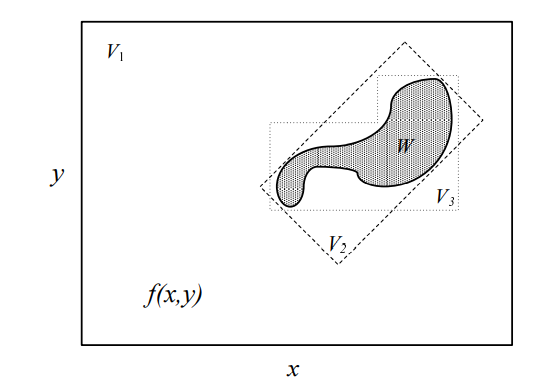
\includegraphics[width=.60\textwidth]{Montecarlo integration.PNG}}
\caption{}
\label{fig:Rejection method1}
\end{figure}

%\clearpage
\subsubsection{Importance Sampling: (da completare MATIAS)}
NB SEE PG 411 NUM REC

The volume in an hypercube is concentrated in it's outer part and is given by:
\[ V(L,n)=L^{n}\]
thus:
\[\Delta V = V(L,n) - V(L-\delta,n)\]
this implies
\[ \frac{\Delta V}{V}\sim n\frac{\delta}{L}\]
which proove the assertion that the fraction of volume increase clearly with the number of dimension and the the volume gratest part of volume will be located very close to the surface of this hypercube.

How we perform trivial estimation of integral?
We will generate point uniformly distributed in the domain of the function f upon which we are integrating.

continue\\ 
In more than three dimension integration over a Volume will become less efficient for the fact we had already mentioned. No points will be generated on the boundary of the hypercube which is the most important.

Suppose that an integrand f can be written as the product of a function h that is almost constant times another, positive, function g. Then its integral over a multidimensional volume V is:
\[\int fdV=\int\frac{f}{g}\cdot gdV = \int hgdV\]

\[I=\int f dV= \int \frac{f}{p} \cdot p dV= mean(\frac{f}{p})V \pm V\cdot Var(\frac{f}{p}) = \]
in this way we are improving the generation 

\[Var(f)= \sqrt{\frac{\langle f^2 \rangle- \langle f  \rangle^2}{N}}\]

\paragraph{The problem of correlation and Variance: How to generated an uncorrelated sample?}


Following formula is denominated partial correlation
\[\hat{R}(k)=\frac{1}{(n-k)\sigma^2}\sum^{n-k}_{t=1}\Big(X_{t}-\mu\Big)\Big(X_{t+k}-\mu\Big) \]
where for k=0 $\hat{R}(k)=1$

if i generate points using metropolis i might use a delta which gives points that are too close to each other.

\begin{figure}[h!t]
\centering
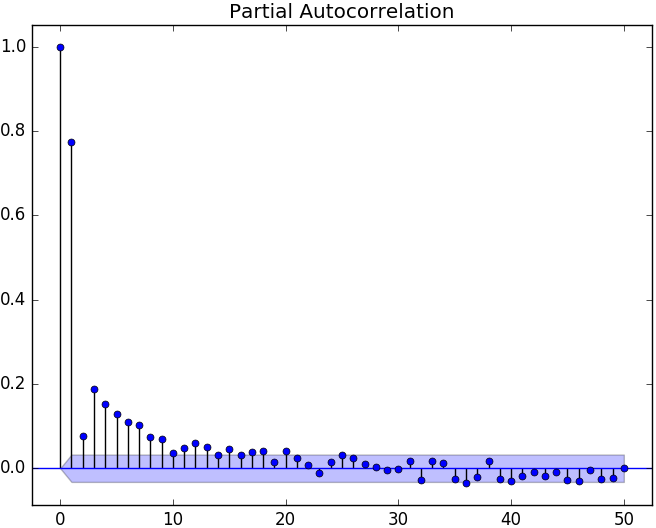
\includegraphics[scale=0.5]{Partial Autocorrelation}
\caption{}\label{PartialAutocorrelation}
\end{figure}